% -*- mode: latex-mode; TeX-engine: xetex; LaTeX-command-style: (("" "SOURCE_DATE_EPOCH=0 %(PDF)%(latex) --shell-escape %S%(PDFout)")); TeX-master: "../dissertation.tex"; -*-

\chapter{Raman sideband cooling}

\section{Theory}

\ref{fig:na-rsc-schematics}

\begin{figure}
  \centering
  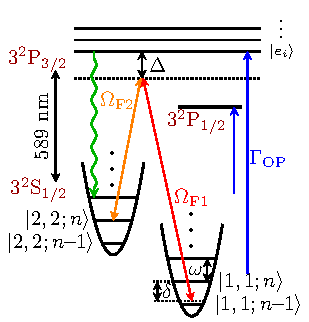
\includegraphics[width=8cm]{figures/na_rsc_schematics.pdf}
  \caption[Schematics of Raman sideband cooling for Sodium.]{
    Single Na atom Raman sideband cooling scheme.
    The Raman transitions between $|2,2;n\rangle$ and $|1,1;n+\Delta n\rangle$
    have a one-photon detuning $\Delta=75$ GHz below the $3^2S_{1/2}$ to $3^2P_{3/2}$ transition.
    Two-photon detuning, $\delta$, is defined relative to the $\Delta n=0$ carrier transition.
    For optical pumping, we use two $\sigma^+$ polarized transitions,
    one to pump the atom state out of $|1,1\rangle$ via $3^2P_{3/2}$
    and one to pump atoms out of $|2,1\rangle$ via $3^2P_{1/2}$
    to minimize heating of the $|2,2\rangle$ state.
    \label{fig:na-rsc-schematics}}
\end{figure}

\section{Setup}

\ref{fig:na-rsc-geometry}

\begin{figure}
  \centering
  \includegraphics[width=8cm]{figures/na_rsc_geometry.pdf}
  \caption[Beams and field geometry for Sodium Raman sideband cooling]{
    Geometry and polarizations of the Raman and optical pumping beams relative to the
    optical tweezer and bias magnetic field.
    Raman beams R1 and R4 address the radial $x$-mode.
    R1 and R2 address the radial $y$-mode.
    R3 and R4 address the axial $z$-mode, where the beams also couple to radial motion,
    but this coupling can be neglected when the atoms is cooled to the ground state of motion.
    \label{fig:na-rsc-geometry}}
\end{figure}

\section{Challenge with large Lamb-Dicky parameter}

\section{Solution: High order sidebands}

\section{Solution: Simulation based optimization}

\section{Cooling performance}
